\documentclass{article}
\usepackage{amsthm,amsmath,amsfonts,lipsum}
\usepackage[T1]{fontenc}
\usepackage{beramono}
\usepackage{listings}
\usepackage{fontawesome5}
\usepackage{adjustbox}
\usepackage{mathabx}
\usepackage{thmtools}
\usepackage{import}
\usepackage{graphicx}
\usepackage{setspace}
\usepackage{geometry}
\usepackage{physics}
\usepackage{float}
\usepackage[english]{babel}
\usepackage{framed}
\usepackage[dvipsnames,x11names]{xcolor}
\usepackage{tcolorbox}
\usepackage{fancyhdr}
\usepackage{hyperref}
\usepackage{booktabs}
\usepackage{enumitem}
\usepackage{cancel}
\usepackage{background}
\usepackage{units}

% Configuring the background
\backgroundsetup{
  scale=1, % Optional, scale if needed
  color=black, % Optional, set the image color, can be omitted
  opacity=0.18, % Optional, adjust opacity for watermark effect
  angle=0,
  position=current page.center, % Center the image on the page
  contents={
\includegraphics[width=1.75\paperwidth, height=1.75\paperheight, keepaspectratio]{ninym_ralei_leaf (watermarked by AlexanderTheMango)}} % Keeps aspect ratio and scales to fill the page
}

% Colours
\definecolor{darkgreen}{rgb}{0.0, 0.5, 0.0}
\definecolor{Firebrick}{rgb}{0.698, 0.132, 0.203}
\definecolor{Crimson}{rgb}{0.862745, 0.078431, 0.235294} % Crimson color
\definecolor{lightred}{rgb}{1.0, 0.819608, 0.819608} % Light red for background

% Define custom tcolorbox styles for notes
\tcbuselibrary{skins, breakable}
\newtcolorbox{definitionbox}{colframe=RoyalBlue, colback=blue!5!white, title=Definition}
\newtcolorbox{examplebox}{colframe=ForestGreen, colback=green!5!white, title=Example}
\newtcolorbox{notebox}{colframe=RedOrange, colback=orange!5!white, title=Note}
\newtcolorbox{theorembox}{colframe=RoyalPurple, colback=purple!5!white, title=Theorem}

\newtcolorbox{propositionbox}{colframe=Goldenrod, colback=yellow!10!white, title=Proposition}
\newtcolorbox{remarkbox}{colframe=MidnightBlue, colback=blue!10!white, title=Remark}
\newtcolorbox{corollarybox}{colframe=OliveGreen, colback=green!10!white, title=Corollary}
\newtcolorbox{warningbox}{colframe=Crimson, colback=lightred, title=Warning}
\newtcolorbox{proofbox}{colframe=Black, colback=gray!10!white, title=Proof}
\newtcolorbox{questionbox}{colframe=Teal, colback=teal!10!white, title=Question}
\newtcolorbox{tipbox}{colframe=Goldenrod, colback=yellow!10!white, title=Tip}
\newtcolorbox{exercisebox}{colframe=darkgreen, colback=green!5!white, title=Exercise}
\newtcolorbox{solutionbox}{colframe=DodgerBlue4, colback=blue!5!white, title=Solution}
\newtcolorbox{algorithmbox}{colframe=Navy, colback=blue!10!white, title=Algorithm}
\newtcolorbox{conceptbox}{colframe=Chocolate, colback=brown!10!white, title=Concept}
\newtcolorbox{illustrationbox}{colframe=Firebrick, colback=red!10!white, title=Illustration}
\newtcolorbox{intuitionbox}{colframe=MediumPurple, colback=purple!10!white, title=Intuition}

% Geometry settings
\geometry{letterpaper, portrait, includeheadfoot=true, hmargin=1in, vmargin=1in}
\onehalfspacing

% Header and footer
\pagestyle{fancy}
\fancyhf{}
\lhead{MAT232 - Lecture Notes}
\rhead{\thepage}
\lfoot{University of Toronto Mississauga}
\rfoot{\today}

% Document starts
\begin{document}
\renewcommand{\familydefault}{\rmdefault}

\begin{titlepage}
    \null % This is a TeX command that does nothing but is necessary for vfill to work correctly
    \vfill
    \begin{center}
        {\fontsize{40}{48}\selectfont \bfseries MAT232 - Lecture 13}
        \vspace{20pt} \\
        {\LARGE after partial derivatives?} \\
        \vspace{20pt}
        \textbf{AlexanderTheMango}
        \vspace{8pt}
        \\ Prepared for February 24, 2025
    \end{center}
    \vfill
\end{titlepage}

\normalsize

\begin{titlepage}
    \null % Ensures proper alignment with vfill
    \vfill
    \begin{center}
        {\Huge \textbf{Definitions and Theorems}} \\[20pt]
        \rule{\textwidth}{0.5mm} \\[15pt]
        {\Large \textit{Straight from the textbook — lots of fluff this time, more than what we need!}} \\[15pt]
        \rule{\textwidth}{0.5mm} \\[15pt]
        \textbf{Quick recap before diving into the lecture.}
    \end{center}
    \vfill
\end{titlepage}

\section*{Parametric Equations and Parameters}

\begin{definitionbox}
If \( x \) and \( y \) are continuous functions of \( t \) on an interval \( I \), then the equations  
\[
x = x(t) \quad \text{and} \quad y = y(t)
\]  
are called \textbf{parametric equations}, and \( t \) is called the \textbf{parameter}. The set of points \( (x, y) \) obtained as \( t \) varies over the interval \( I \) is called the \textbf{graph of the parametric equations}. The graph of parametric equations is referred to as a \textbf{parametric curve} or \textbf{plane curve}, and is denoted by \( C \).  
\end{definitionbox}

\section*{Theorem 1.1: Derivative of Parametric Equations}
\begin{theorembox}
Consider the plane curve defined by the parametric equations \( x = x(t) \) and \( y = y(t) \). Suppose that \( x'(t) \) and \( y'(t) \) exist, and assume that \( x'(t) \neq 0 \). Then the derivative \( \frac{dy}{dx} \) is given by  
\[
\frac{dy}{dx} = \frac{\frac{dy}{dt}}{\frac{dx}{dt}} = \frac{y'(t)}{x'(t)}.
\]
\begin{proofbox}
    \begin{proof}
    \leavevmode\\
        This theorem can be proven using the Chain Rule. Assume that the parameter \( t \) can be eliminated, yielding a differentiable function \( y = F(x) \). Then \( y(t) = F(x(t)) \). Differentiating both sides of this equation using the Chain Rule gives  
        \[
        y'(t) = F'(x(t)) x'(t),
        \]  
        so  
        \[
        F'(x(t)) = \frac{y'(t)}{x'(t)}.
        \]  
        But \( F'(x(t)) = \frac{dy}{dx} \), which proves the theorem. \\
    \end{proof}
    \end{proofbox}
\end{theorembox}

\section*{Equation 1.1 and Applications}
\begin{notebox}
Equation 1.1 can be used to calculate derivatives of plane curves, as well as critical points. Recall that a critical point of a differentiable function \( y = f(x) \) is any point \( x = x_0 \) such that either \( f'(x_0) = 0 \) or \( f'(x_0) \) does not exist. Equation 1.1 gives a formula for the slope of a tangent line to a curve defined parametrically regardless of whether the curve can be described by a function \( y = f(x) \) or not.
\end{notebox}

\section*{Second-Order Derivatives}
\begin{theorembox}
The next goal is to see how to take the second derivative of a function defined parametrically. The second derivative of a function \( y = f(x) \) is defined to be the derivative of the first derivative; that is,  
\[
\frac{d^2y}{dx^2} = \frac{d}{dx} \left[ \frac{dy}{dx} \right].
\]  

Since \( \frac{dy}{dx} = \frac{\frac{dy}{dt}}{\frac{dx}{dt}} \), it is possible to replace \( y \) on both sides of this equation with \( \frac{dy}{dx} \). This yields
\[
\frac{d^2y}{dx^2} = \frac{\frac{d}{dt}\left( \frac{dy}{dx} \right)}{\frac{dx}{dt}}.
\]
\end{theorembox}

\begin{titlepage}
    \null % Ensures proper alignment with vfill
    \vfill
    \begin{center}
        {\Huge \textbf{Let’s Get Started}} \\[20pt]
        \rule{\textwidth}{0.5mm} \\[15pt]
        {\Large \textit{Time to dive into the lecture notes.}} \\[15pt]
        \rule{\textwidth}{0.5mm} \\[15pt]
        \textbf{Grab your pen or pencil, and let’s break this down step by step.}
    \end{center}
    \vfill
\end{titlepage}


\section*{Key Concept}
\begin{definitionbox}
A \textbf{parametric equation} is a set of equations that express the coordinates of the points of a curve as functions of a variable, called a parameter.
\end{definitionbox}

\section*{Sketching Parametric Equations}
\begin{examplebox}
\textbf{Example:} Sketch the graph, using a table of values:
\[ x = t + \frac{1}{t}, \quad y = t - \frac{1}{t}, \quad t > 0. \]
\begin{solutionbox}
    \textbf{Table of Values:}
\begin{center}
\begin{adjustbox}{max width=\textwidth, max height=\textheight}
\large
\begin{tabular}{|c|c|c|c|}
\hline
$t$    & $1/t$ & $x$ & $y$ \\ \hline
$0.01$ & $\nicefrac{1}{0.01} = \nicefrac{1}{\frac{1}{100}} = 100$     & $100.01$   & $0.01 - 100 = -99.99$   \\ \hline
$0.1$  & $\nicefrac{1}{0.1} = \nicefrac{1}{\frac{1}{10}} = 10$     & $10.1$   & $-9.9$   \\ \hline
$0.2$  & $\nicefrac{1}{0.2} = \nicefrac{1}{\frac{20}{100}} = \nicefrac{1}{\frac{2}{10}} = 5$     & $5.2$   & $4.8$   \\ \hline
$1$    & $\frac{1}{1}$     & $2$   & $0$   \\ \hline
$5.0$  & $0.2$     & $5.2$   & $4.8$   \\ \hline
$10$   & $0.1$     & $10.1$   & $9.9$   \\ \hline
$10$   & $0.01$    & $100.01$   & $99.99$   \\ \hline
\end{tabular}
\normalsize
\end{adjustbox}
\end{center}
\begin{figure}[H]
    \centering
    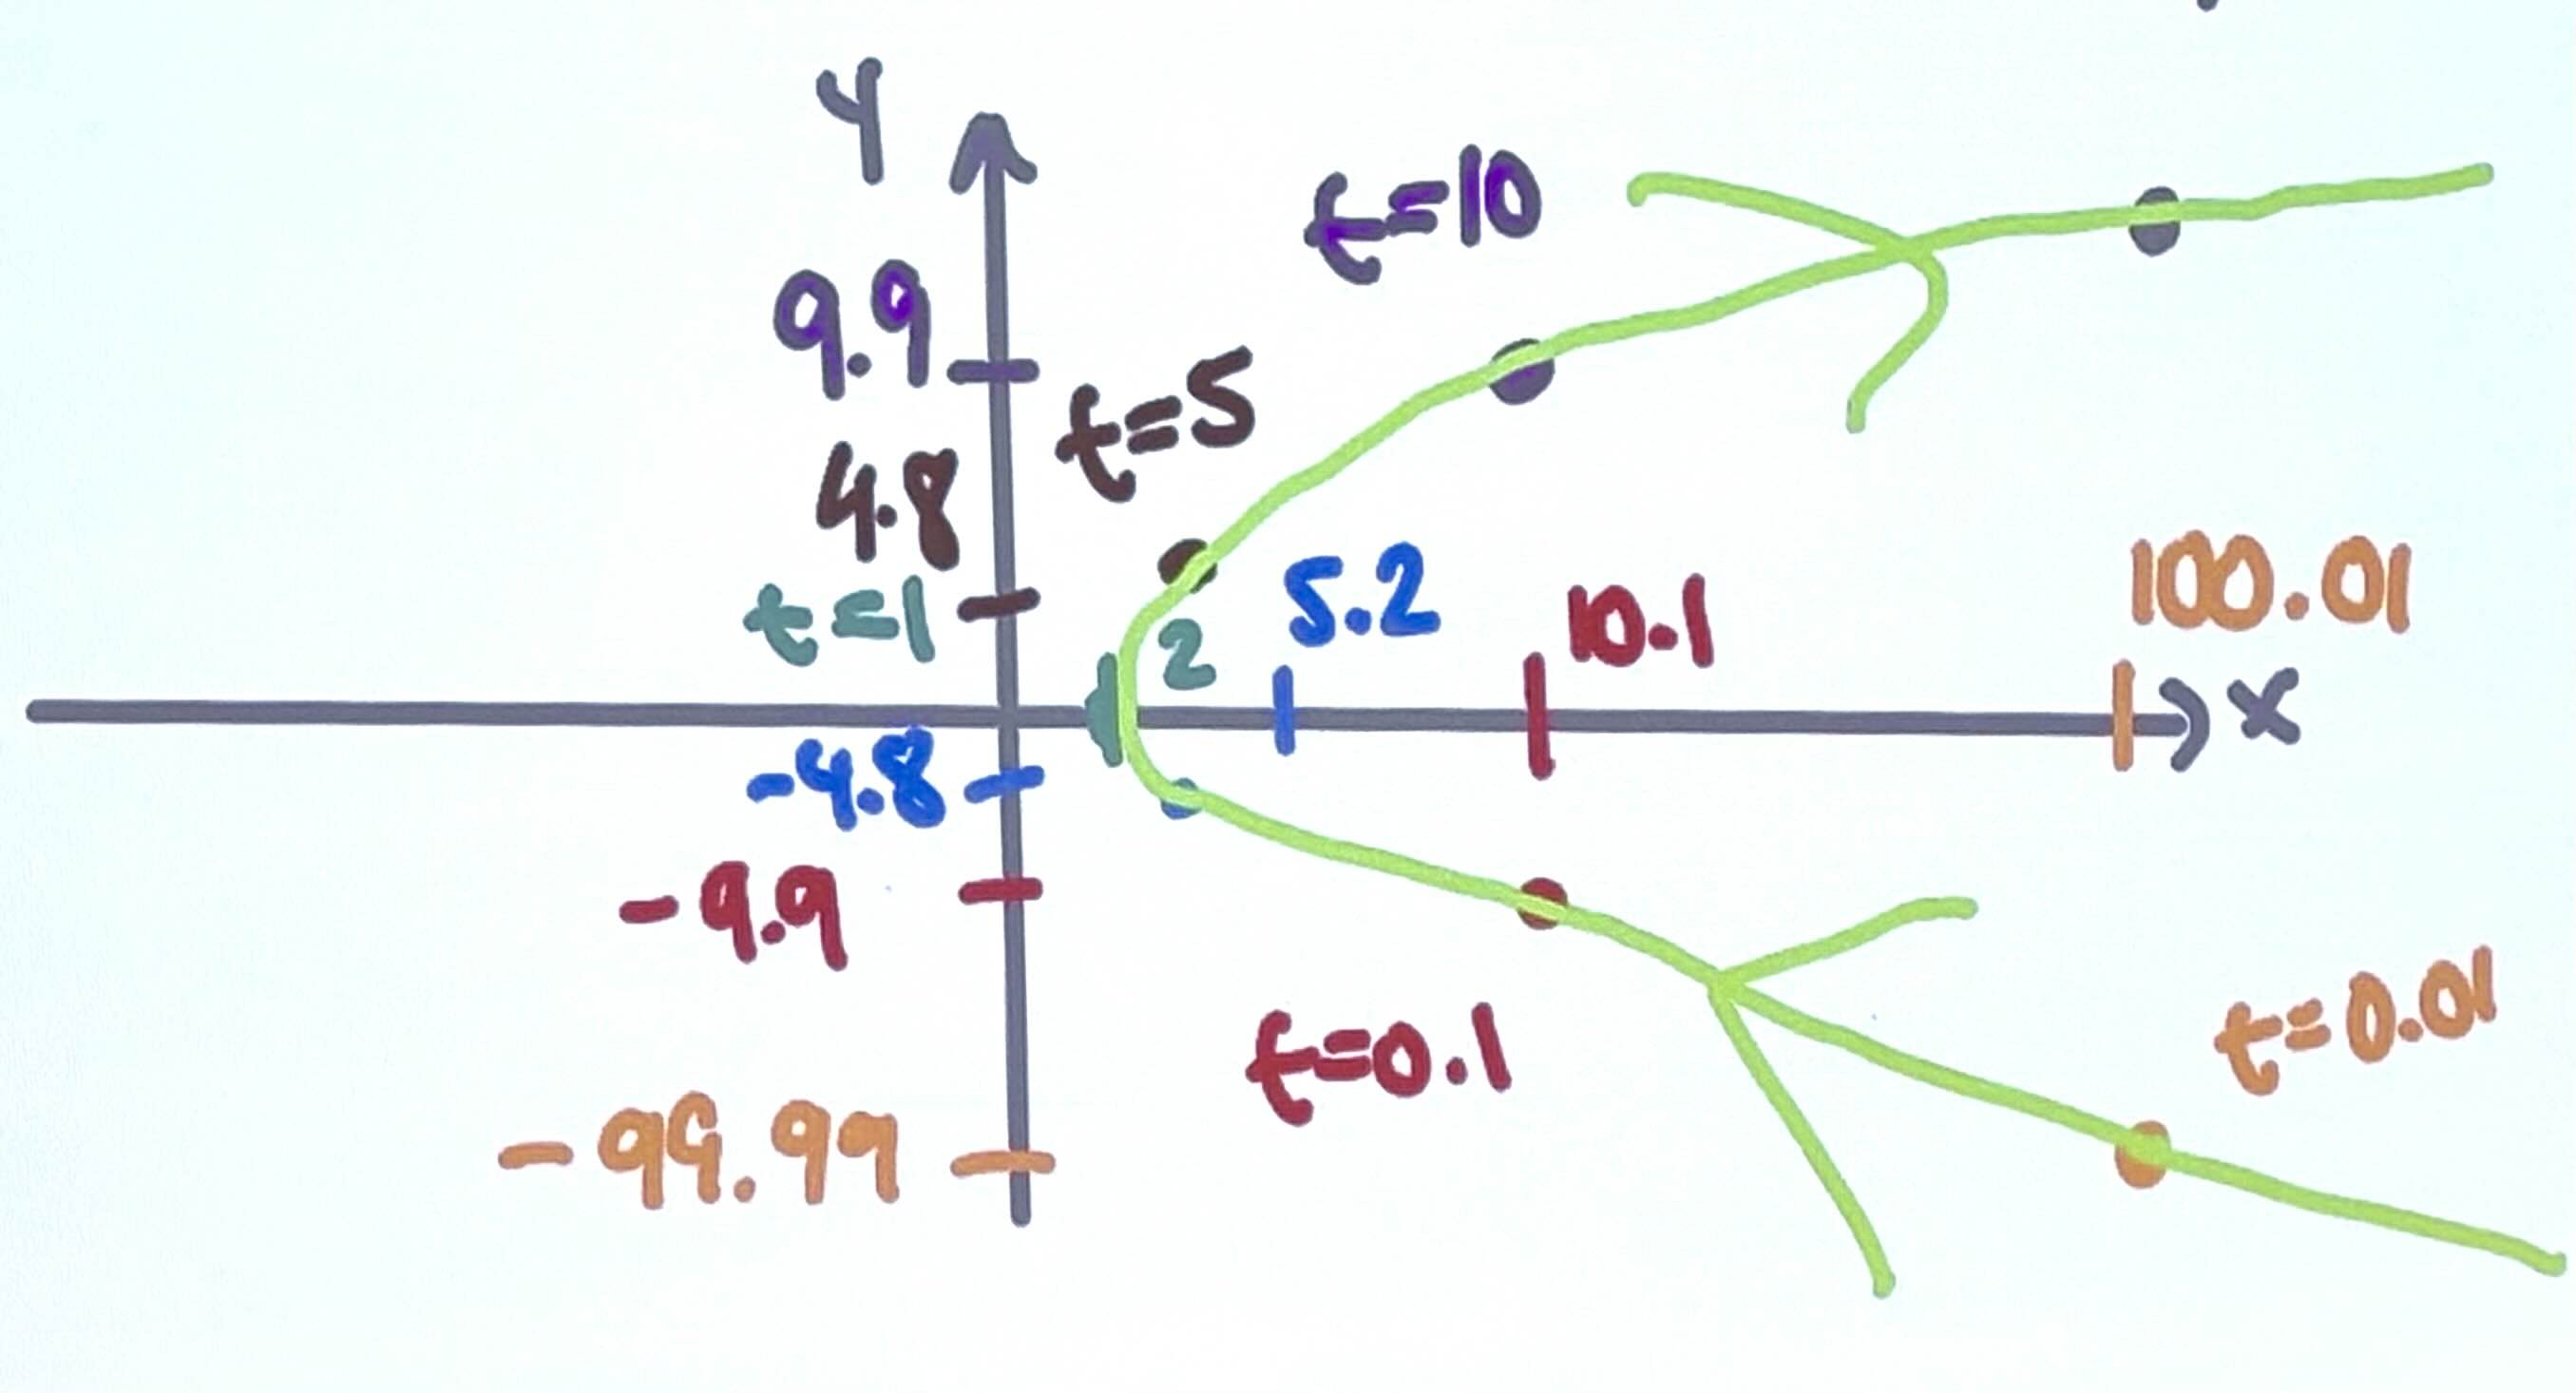
\includegraphics[width=0.5\textwidth]{hyperbola.jpg}
    \caption{The corresponding hyperbolic graph.}
    \label{fig:sample_image}
\end{figure}
\end{solutionbox}
\end{examplebox}

\begin{examplebox}
\textbf{Example:} Sketch the graph of the same parametric equation, using the elimination method:
\[
x = t + \frac{1}{t}, \quad y = t - \frac{1}{t}, \quad t > 0.
\]

\begin{solutionbox}
    We start by simplifying the expressions for \( x \) and \( y \):
    
    \[
    \text{LHS} = A^2 - B^2 = (A - B)(A + B) = \text{RHS}.
    \]
    Let \( A = x \) and \( B = y \), so we can rewrite this as:
    \[
    \text{LHS:} \quad x^2 - y^2.
    \]
    
    Now, compute \( A - B \) and \( A + B \):
    
    \[
    A - B = x - y = \left( t + \frac{1}{t} \right) - \left( t - \frac{1}{t} \right) = \frac{2}{t},
    \]
    \[
    A + B = x + y = \left( t + \frac{1}{t} \right) + \left( t - \frac{1}{t} \right) = 2t.
    \]
    
    Now, calculate the RHS:
    \[
    \text{RHS:} \quad (A - B)(A + B) = (x - y)(x + y) = \left( \frac{2}{t} \right)(2t) = 4.
    \]
    
    Thus, we obtain the equation:
    \[
    x^2 - y^2 = 4, \quad x > 0.
    \]

    \begin{figure}[H]
    \centering
    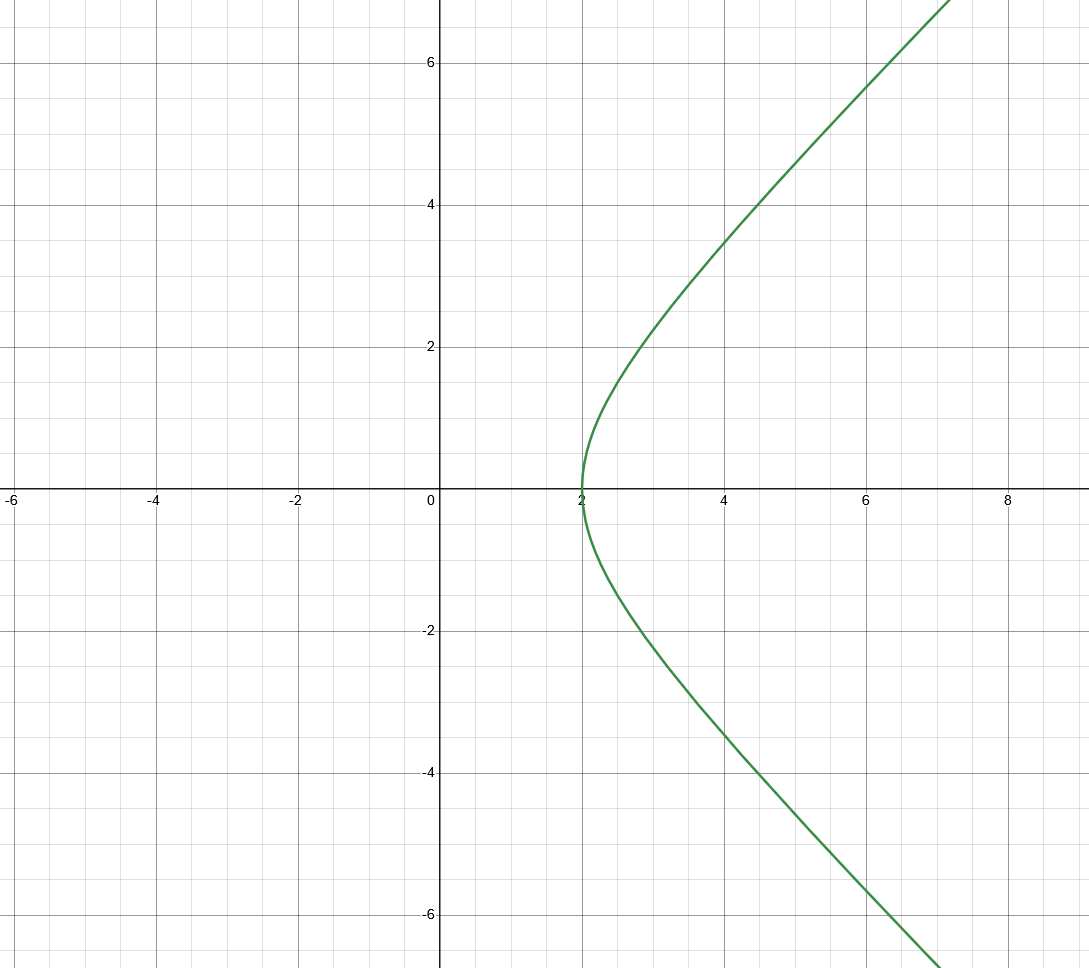
\includegraphics[width=0.35\textwidth]{hyperbola_nicer.jpg}
    \caption{Precise graph of the parametric equation \( x = t + \frac{1}{t}, \quad y = t - \frac{1}{t}, \quad x > 0 \)}
    \end{figure}
\end{solutionbox}    
\end{examplebox}    

\section*{The Slope of a Parametric Curve}

\begin{definitionbox}
\textbf{Definition:} If \( x(t) \) and \( y(t) \) are differentiable functions, the slope of the curve described by these parametric equations is given by:  
\[
\frac{dy}{dx} = \frac{\frac{dy}{dt}}{\frac{dx}{dt}}, \quad \text{provided } \frac{dx}{dt} \neq 0.
\]
\begin{remarkbox}
    This formula allows you to find the slope of the tangent line to the curve at any point where the derivative of \( x(t) \) with respect to \( t \) is nonzero. \\
    \\
    Here's a concrete example illustration!
    \begin{figure}[H]
        \centering
        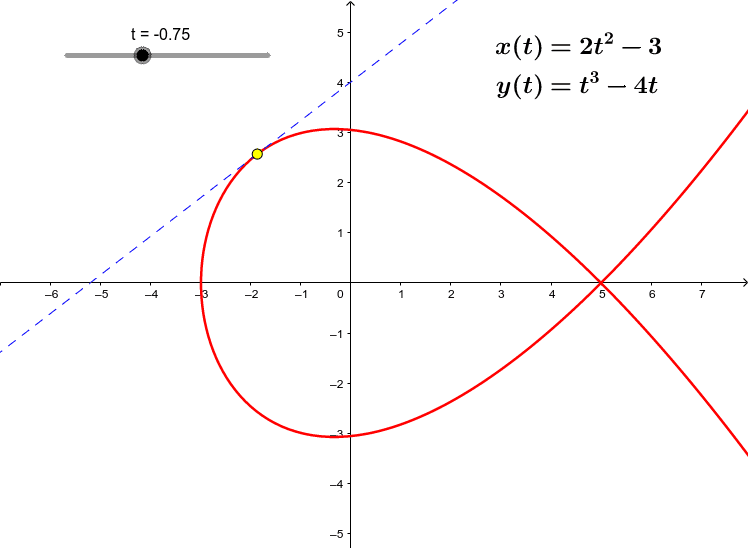
\includegraphics[width=0.6\textwidth]{slopeparametricexample.png}
        \caption{Graphical representation of the slope of a parametric curve.}
        \label{fig:slopeparametricexample}
    \end{figure}
\end{remarkbox}
\end{definitionbox}

\section*{Parametric Curve Sketching Practice Questions}

\begin{exercisebox}
\textbf{Question 1:} Sketch and eliminate \( t \) if possible: \\
\[
    x = t^2, \quad y = t^3, \quad -2 \leq t \leq 2
\]
Note that this is a closed interval, which means the graph starts at \( t = -2 \) and ends at \( t = 2 \). The starting point is where \( t = -2 \), and the finishing point is where \( t = 2 \). The direction of the graph should be indicated using an arrow as \( t \to 2 \).

Express the relationship between \( x \) and \( y \) in Cartesian form.

\begin{solutionbox}
    \textbf{Solution:}
    
    The parametric equations are \( x = t^2 \) and \( y = t^3 \). We aim to eliminate \( t \).
    
    From \( x = t^2 \), we can solve for \( t \) as:
    \[
        t = \pm \sqrt{x}.
    \]
    Substituting this into the equation for \( y \):
    \[
        y = (\pm \sqrt{x})^3 = \pm x^{3/2}.
    \]
    Thus, the Cartesian form is:
    \[
        y = \pm x^{3/2}.
    \]
    This describes a curve that is symmetric about the x-axis. The graph starts at \( t = -2 \) with coordinates \( (x, y) = (4, -8) \), and ends at \( t = 2 \) with coordinates \( (x, y) = (4, 8) \). The graph is symmetric, opening upwards and downwards, as \( t \) moves from \( -2 \) to \( 2 \).
    
    As \( t \) increases, the direction of the graph is indicated by the arrows as shown below.
    
    \begin{figure}[H]
        \centering
        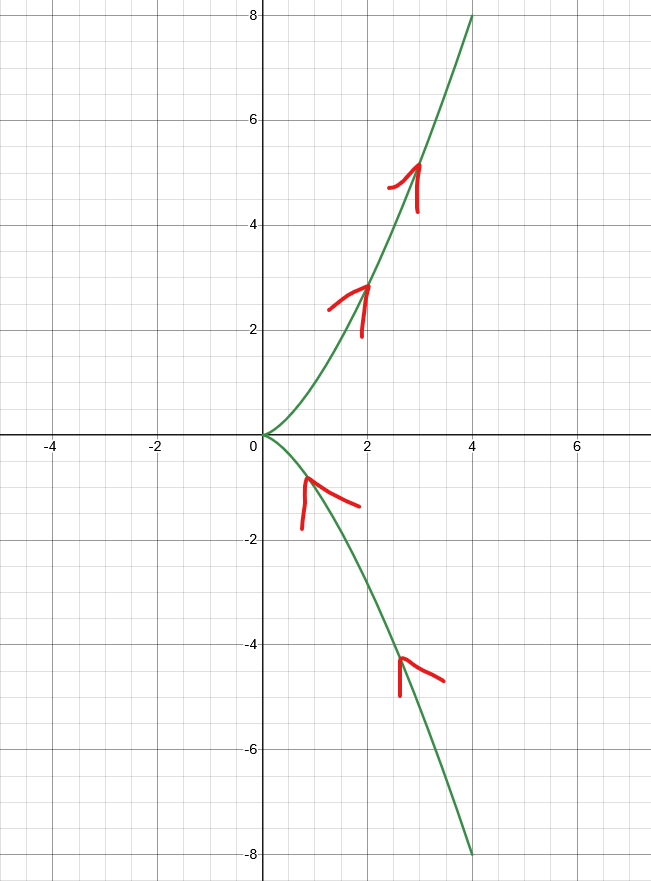
\includegraphics[width=0.22\textwidth]{curvesketchingpractice1.png}
        \caption{Graph of the curve for \( x = t^2, y = t^3 \).}
        \label{fig:curvesketchingpractice1}
    \end{figure}
\end{solutionbox}
\end{exercisebox}

\begin{exercisebox}
\textbf{Question 2:} Sketch and eliminate \( t \) if possible for each of the following parametric equations:

\[
    c_1: x = -\cos\left(\frac{t}{4}\right), \quad y = \sin\left(\frac{t}{4}\right), \quad 0 \leq t \leq 4\pi
\]
\[
    c_2: x = -\sin(t), \quad y = -\cos(t), \quad \frac{\pi}{2} \leq t \leq \frac{3\pi}{2}
\]
\[
    c_3: x = \cos(t), \quad y = \sin(t), \quad t \in [0, \pi]
\]
For each equation, express the relationship in Cartesian form and sketch the curve. The hint suggests that \( x = r \cos(\theta) \), \( y = r \sin(\theta) \), and \( x^2 + y^2 = r^2 \). For these curves, \( r = 1 \).

\begin{solutionbox}
    \textbf{Solution} \textit{(see illustration below)}\textbf{:}
    
    \textbf{For \( c_1 \):}
    The parametric equations are \( x = -\cos\left(\frac{t}{4}\right) \) and \( y = \sin\left(\frac{t}{4}\right) \). To eliminate \( t \), use the identity \( \cos^2\theta + \sin^2\theta = 1 \), where \( \theta = \frac{t}{4} \). This gives:
    \[
        x^2 + y^2 = \cos^2\left(\frac{t}{4}\right) + \sin^2\left(\frac{t}{4}\right) = 1.
    \]
    This represents a circle with radius 1, centered at the origin.
    
    For \( t = 0 \), we have \( (x, y) = (-1, 0) \). For \( t = 4\pi \), we have \( (x, y) = (1, 0) \). The curve traces a semicircle in the clockwise direction, starting at \( -1, 0 \) and ending at \( (1, 0) \).
    
    \textbf{For \( c_2 \):}
    The parametric equations are \( x = -\sin(t) \) and \( y = -\cos(t) \). Using the identity \( \sin^2\theta + \cos^2\theta = 1 \), we have:
    \[
        x^2 + y^2 = \sin^2(t) + \cos^2(t) = 1.
    \]
    This describes a unit circle. The curve starts at \( t = \frac{\pi}{2} \), corresponding to \( (x, y) = (-1, 0) \), and ends at \( t = \frac{3\pi}{2} \), corresponding to \( (x, y) = (1, 0) \). The graph traces a semicircle in the clockwise direction.
    
    \textbf{For \( c_3 \):}
    The parametric equations are \( x = \cos(t) \) and \( y = \sin(t) \). Again using the identity \( \cos^2\theta + \sin^2\theta = 1 \), we get:
    \[
        x^2 + y^2 = \cos^2(t) + \sin^2(t) = 1.
    \]
    This describes a unit circle. The curve starts at \( t = 0 \), corresponding to \( (x, y) = (1, 0) \), and ends at \( t = \pi \), corresponding to \( (x, y) = (-1, 0) \). The graph traces the upper half of the unit circle, moving counterclockwise.
\end{solutionbox}
\end{exercisebox}

\begin{illustrationbox}
    \begin{figure}[H]
        \centering
        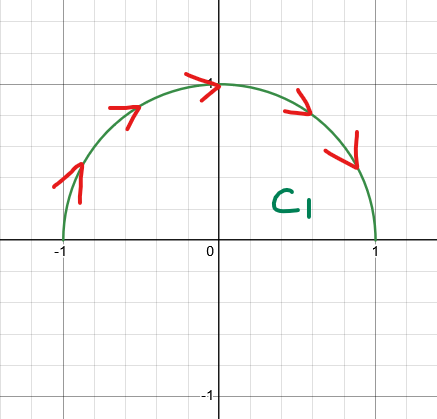
\includegraphics[width=0.4\textwidth]{c1.png}
        \caption{Graph of the curve for \( c_1 \).}
        \label{fig:curvesketchingpractice2}
    \end{figure}
    \begin{figure}[H]
        \centering
        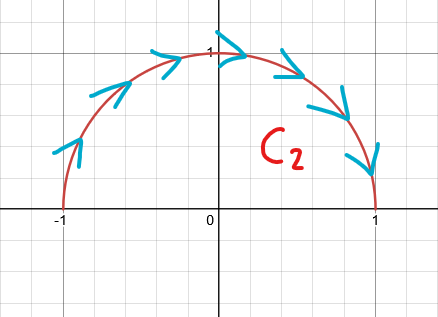
\includegraphics[width=0.4\textwidth]{c2.png}
        \caption{Graph of the curve for \( c_2 \).}
        \label{fig:curvesketchingpractice2}
    \end{figure}
    \begin{figure}[H]
        \centering
        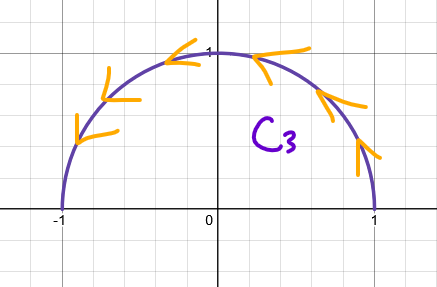
\includegraphics[width=0.4\textwidth]{c3.png}
        \caption{Graph of the curve for \( c_3 \).}
        \label{fig:curvesketchingpractice2}
    \end{figure}
\end{illustrationbox}

\section*{The Elimination Method Does NOT Always Work}
\begin{warningbox}
    In some cases, it is not possible to eliminate the parameter \( t \) to express the relationship between \( x \) and \( y \) in a Cartesian form. While elimination works in many situations—especially when the parametric equations describe simpler curves, like circles or straight lines—there are cases where it's not possible to eliminate \( t \) algebraically, or it becomes extremely complicated to do so. 
    
    \subsection*{Example:}
    
    Consider the following parametric equations:
    \[
    x = e^t - \sin^2(t), \quad y = \ln(t) + \frac{1}{t}, \quad t > 0
    \]
    
    - Here, \( x \) and \( y \) are both expressed in terms of \( t \), but neither \( x \) nor \( y \) is simply related to \( t \) in a way that allows for easy elimination of \( t \).
    
    \subsection*{Why Can't We Eliminate \( t \)?}
    
    Let's break down why we can't eliminate \( t \) easily from these equations.
    
    \begin{itemize}
        \item \textbf{The equation for \( x \)}:
        \[
        x = e^t - \sin^2(t)
        \]
        This equation involves both an exponential function (\( e^t \)) and a trigonometric function (\( \sin^2(t) \)), making it nontrivial to solve for \( t \) in terms of \( x \). The combination of these two types of functions—one that grows exponentially and another that oscillates—does not lead to a simple relationship between \( x \) and \( t \).
        
        \item \textbf{The equation for \( y \)}:
        \[
        y = \ln(t) + \frac{1}{t}
        \]
        This equation involves a logarithmic function (\( \ln(t) \)) and a rational function (\( \frac{1}{t} \)). Again, these are not straightforward to combine algebraically to eliminate \( t \), as the presence of \( t \) in different forms (in the logarithmic and rational terms) complicates the process.
    \end{itemize}
    
    \subsection*{The Resulting Complexity}
    
    To try and eliminate \( t \), we would have to manipulate these equations in such a way that we express one variable in terms of the other, without involving \( t \). However, due to the combination of different types of functions (exponential, trigonometric, logarithmic, and rational), it becomes extremely difficult to isolate \( t \) in either equation and then substitute it into the other equation.
    
    In this case, even if we tried solving one equation for \( t \) and substituting it into the other, the resulting expressions would likely be too complicated or may not even have a simple closed form.
    
    \subsection*{Conclusion}
    
    The \textbf{elimination method} relies on being able to algebraically manipulate the parametric equations into a form where we can solve for \( t \) and eliminate it. However, in cases like this one, where the parametric equations involve complex combinations of different types of functions (like exponentials, trigonometric functions, and logarithms), the elimination method becomes impractical or impossible.
    
    This is why the elimination method does not always work, and in these situations, it's important to either:
    \begin{itemize}
        \item \textbf{Graph the parametric equations} to understand the curve visually, or
        \item Use other methods such as \textbf{numerical techniques} or \textbf{approximation methods} if a Cartesian form is needed.
    \end{itemize}    
\end{warningbox}

\section*{Further Visualization}
\begin{figure}[H]
    \centering
    
\includegraphics[width=0.6\textwidth]{sample_image2.jpg}
    \caption{Additional visualization for parametric curves.}
    \label{fig:sample_image2}
\end{figure}

\section*{Section 1.2: Calculus on Parametric Equations}
\section*{Key Concepts}
Recall the concept from $1^{\text{st}}$ year calculus:
\begin{definitionbox}
If \( y = f(x) \) is given, then the slope of the tangent line to the curve of \( y = f(x) \) is:
\[
    y' = f'(x) = \frac{dy}{dx}
\]
\end{definitionbox}
Now, for MAT232, we have:
\begin{definitionbox}
Given \( x = f(t), \quad y = g(t), \quad t \in \mathbb{R} \), these are defifferentiable w.r.t.\ (w.r.t.\ = ``with respect to'') \( t \). This is such that:
\[
    \frac{dy}{dx} = \frac{\frac{dy}{dt}}{\frac{dx}{dt}}, \frac{dx}{dt} \neq 0
\]
This will also be provided in the formula sheet. \\
\\
\[
    x = f(t), \quad y = g(t), \quad t \in \mathbb{R}
\]
Because the chain rule must follow through, always! \\
\textit{Here is the derivation:}
So \dots \( y = g(t) \) \\
\[
     \frac{dy}{dt} = \frac{dy}{dx} \cdot \frac{dx}{dt}
\]
\textit{Chain rule.} \\
\\
\[
    \frac{\frac{dy}{dt}}{\frac{dx}{dt}} = \frac{dy}{dx}, \quad \text{provided that} \quad \frac{dx}{dt} \neq 0
\]
\end{definitionbox}

\section*{Second Derivative}
\begin{theorembox}
Given \( x = f(t), y = g(t), t \in \mathbb{R} \) are differentiable at \( t \) and \( \frac{dy}{dx} = \frac{\frac{dy}{dt}}{\frac{dx}{dt}} \) exists and is differentiable at \( t \):
\[
    \frac{d^{2y}}{dx^2} = \frac{d}{dx}(\frac{dy}{dx}) = dx(\frac{\frac{dy}{dt}}{\frac{dx}{dt}})
\]
Notice that the expression of the innermost bracket is a derivative all in terms of \( t \).
Thus:
\[
    = \frac{d}{dt}(\frac{\frac{dy}{dt}}{\frac{dx}{dt}}) \cdot \frac{dt}{dx} = \frac{d}{dt}(\frac{\frac{dy}{dt}}{\frac{dx}{dt}}) = \frac{\frac{d}{dt}(\frac{\frac{dy}{dt}}{\frac{dx}{dt}})}{\frac{dx}{dt}} \text{.}
\]
This follows from the \textbf{inverse function theorem}. \\
Collectively, it follows that:
\[
    \frac{d^2y}{dx^2} = \frac{\frac{d}{dt}(\frac{\frac{dy}{dt}}{\frac{dx}{dt}})}{\frac{dx}{dt}}, \quad \frac{dx}{dt} \neq 0 \text{.}
\]
\textit{This is not included on the formula sheet.}
\end{theorembox}

\section*{Examples}
\begin{examplebox}
Consider the following parametric curve:
\[
    x = \sec(t), \quad y = \tan(t), \quad -\frac{\pi}{2} < t < \frac{\pi}{2}
\]
(A) Find the tangent line to the given curve at the point \( (\sqrt{2}, 1) \) where \( t = \frac{\pi}{4} \). \\
(B) Find the vertical tangent(s), if any. \\
(C) Find \( \frac{d^2y}{dx^2} \).
\end{examplebox}
Let's do this, one at a time! \\
\\
(A) Find the tangent line to the given curve at the point \( (\sqrt{2}, 1) \) where \( t = \frac{\pi}{4} \).
\begin{examplebox}
\underline{Tangent Line:}
Recall\dots
\begin{enumerate}
    \item \( y - y_0 = m(x - x_0) \), where \( m \) is the slope and \( (x_0, y_0) \) is a point on the curve;
    \item \( y = mx + b \), where \( m \) is the slope and \( b \) is the y-intercept.
\end{enumerate}
Given point \( (\sqrt{2}, 1) = (x_0, y_0) \), \( \frac{dy}{dt} = \sec^2(t) \), and \( \frac{dx}{dt} = \sec(t)\tan(t) \), it follows that:
\[
    m = \frac{dy}{dx} = \frac{\frac{dy}{dt}}{\frac{dx}{dt}} = \frac{\sec^{\cancel{2}}(t)\tan(t)}{\cancel{\sec(t)}\tan(t)} = \frac{\sec(t)}{\tan(t)}
\]
Next, \( \frac{dy}{dx} \mid_{t = \frac{\pi}{4}} = \frac{\sec(\frac{\pi}{4})}{\tan(\frac{\pi}{4})} = \frac{\sqrt{2}}{1} = \sqrt{2} = m \). \\

Remember:
\[
    \sec(\theta) = \frac{1}{\cos(\theta)}
\]
\[
    \csc(\theta) = \frac{1}{\sin(\theta)}
\]
Note that \( \frac{1}{\sqrt{2}} = \frac{\sqrt{2}}{2} \). \\
So\dots
\[
    \sec(\frac{\pi}{4}) = \frac{1}{\cos(\frac{\pi}{4})} = \frac{1}{\frac{1}{\sqrt{2}}} = \sqrt{2}
\]
Tangent Line:
\[
    y - y_0 = m(x - x_0)
\]
\[
    y - 1 = \sqrt{2} (x - \sqrt{2})
\]
\[
    y = \sqrt{2}x - 1
\]
is the tangent line!

\end{examplebox}

(B) Find the vertical tangent(s), if any.
\begin{examplebox}
\[
    \frac{dy}{dt} = \sec^2(t)
\]
\[
    \frac{dx}{dt} = \sec(t)\tan(t)
\]
So\dots
\[
    \frac{dy}{dx} = \frac{\frac{dy}{dt}}{\frac{dx}{dt}} = \frac{\sec^2(t)}{\sec(t)\tan(t)}
\]

Recall from first year calculus:
\begin{theorembox}
    Given \( y = f(x) \), it follows that \( y' = f'(x) = 0 \). That is, the roots of \( y' = 0 \) indicate the positions of the horizontal tangents.
\end{theorembox}
So\dots\\
Horizonal Tangent: \( \frac{dy}{dx} = 0 \); find \( t \) values.
\[
    \frac{dy}{dt} = 0, \quad \text{but } \frac{dx}{dt} \neq 0
\]
Vertical Tangent: \( \frac{dy}{dx} \) is \textit{undefined}; find \( t \) values.
\[
    \frac{dx}{dt} = 0, \quad \text{but} \frac{dy}{dt} \neq 0
\]
In this case, there is a singular point:
\[
    \frac{dx}{dt} = 0 \quad \text{and} \quad \frac{dy}{dt} = 0
\]
Vertical Tangents: \( \frac{dx}{dt} = 0 \), but \( \frac{dy}{dt} \neq 0 \). \\
So\dots
\[
    \frac{dx}{dt} = \sec(t)\tan(t) = 0, \quad -\frac{\pi}{2} < t < \frac{\pi}{2} \text{.}
\]
Notice that
\begin{itemize}
    \item \( \sec(t) = \frac{1}{\cos(t)} = 0 \) is impossible as \( 1 \neq 0 \);
    \item \( \tan(t) = 0 \) occurs at \( t = 0 \).
\end{itemize}
Now, check \( \frac{dy}{dt} = 0 \) at \( t = 0 \).
\[
    \frac{dy}{dt} = \sec^2(t) = 0, \quad \text{for } t = 0
\]
Is this true? \\
\\
Therefore, the vertical tangent is at \( t = 0 \).
\end{examplebox}

(C) Find \( \frac{d^2y}{dx^2} \).
\begin{examplebox}
Recall:
\[
    \frac{d^2y}{dx^2} = \frac{\frac{d}{dt}(\frac{\frac{dy}{dt}}{\frac{dx}{dt}})}{\frac{dx}{dt}}
\]
\[
    \frac{dy}{dx} = \frac{\sec(t)}{\tan(t)} \quad \text{and} \quad \frac{dx}{dt} = \sec(t)\tan(t)
\]
\[
    \frac{d^2y}{dx^2} = \frac{\frac{d}{dt}(\frac{\sec(t)}{\tan(t)})}{\sec(t)\tan(t)}
\]
\[
    \frac{\sec(t)}{\tan(t)} = \frac{\frac{1}{cos(t)}} \cdot {\frac{\sin(t)}{\cos(t)}} = \frac{1}{\cos(t)}(\frac{\cos(t)}{\sin(t)})
\]
\[
    = \frac{1}{\sin(t)}
\]
\[
    \sec(t)\tan(t) = \frac{1}{\cos(t)} \cdot \frac{\sin(t)}{\cos(t)} = \frac{\sin(t)}{\cos^2(t)}
\]
Now, find the derivative of \( y = \frac{1}{\sin(t)}\):
\[
    y' = \frac{0 \cdot \sin(t) - \cos(t) \cdot 1}{\sin^2(t)} = -\frac{\cos(t)}{\sin^2(t)}
\]
\textbf{note to self: finish this off}
\end{examplebox}

\end{document}
